\section*{Question 1}
(1) For each pair ($N$, $h$), the functions ($U$, $f$($U$)), ($U$, $\hat{f}_{h}$($U$)), and the sample points ($x_{k}$, $y_{k}$), where $k$ = 1, ..., $N$, are plotted below in Figures 1 and 2.
\begin{figure}[h!]
    \centering
    \begin{subfigure}[h]{0.5\textwidth}
        \centering
        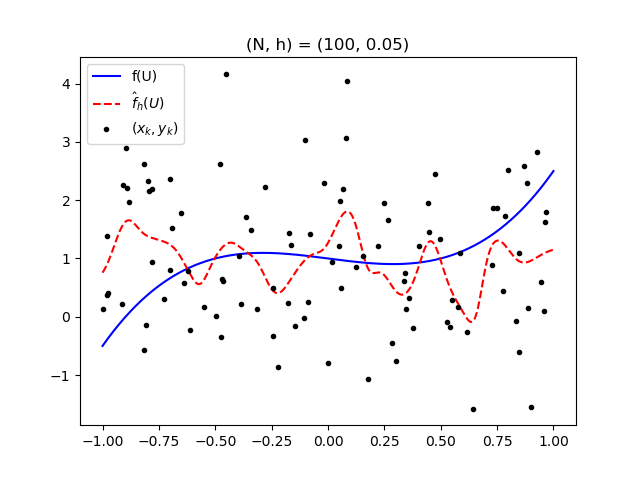
\includegraphics[height=2.4in]{Figure_1.png}
    \end{subfigure}%
    \begin{subfigure}[h]{0.5\textwidth}
        \centering
        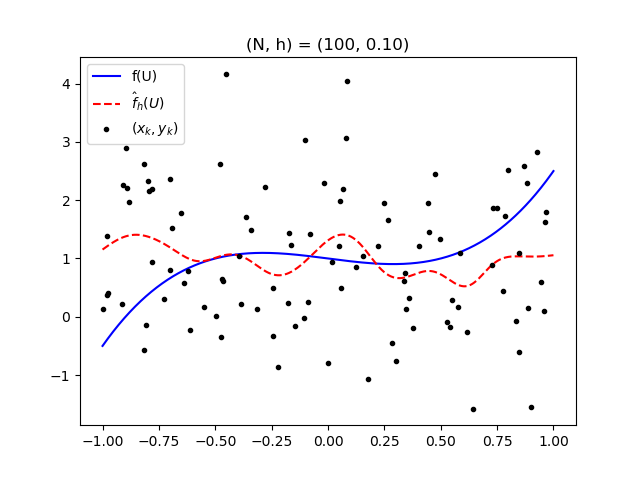
\includegraphics[height=2.4in]{Figure_2.png}
    \end{subfigure}
    \begin{subfigure}[h]{0.5\textwidth}
        \centering
        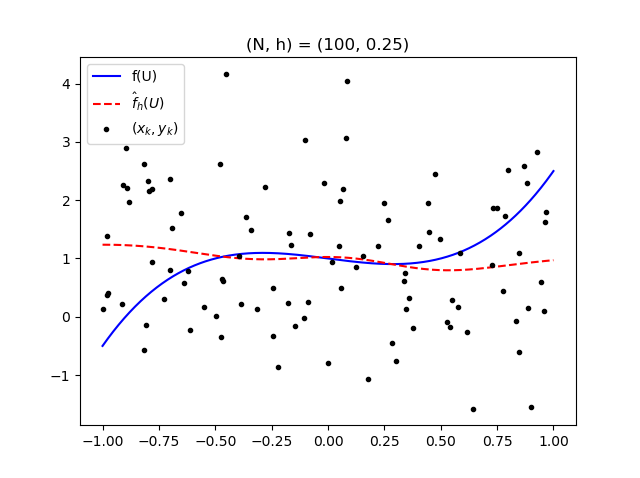
\includegraphics[height=2.4in]{Figure_3.png}
    \end{subfigure}%
    \begin{subfigure}[h]{0.5\textwidth}
        \centering
        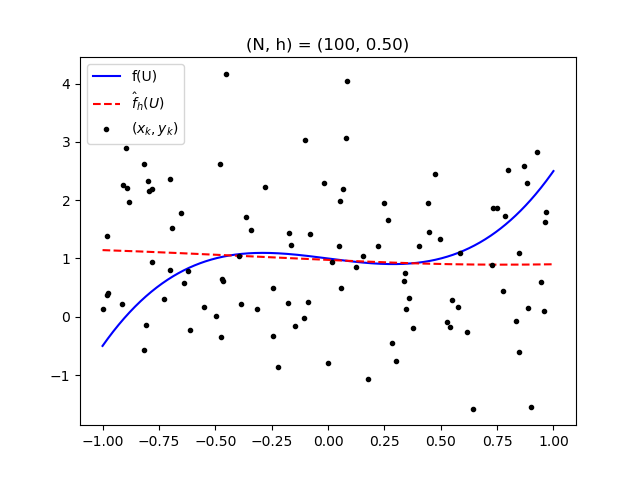
\includegraphics[height=2.4in]{Figure_4.png}
    \end{subfigure}
    \caption{Kernel regression estimators for $N$ = 100}
\end{figure}
\begin{figure}[h!]
    \centering
    \begin{subfigure}[h]{0.5\textwidth}
        \centering
        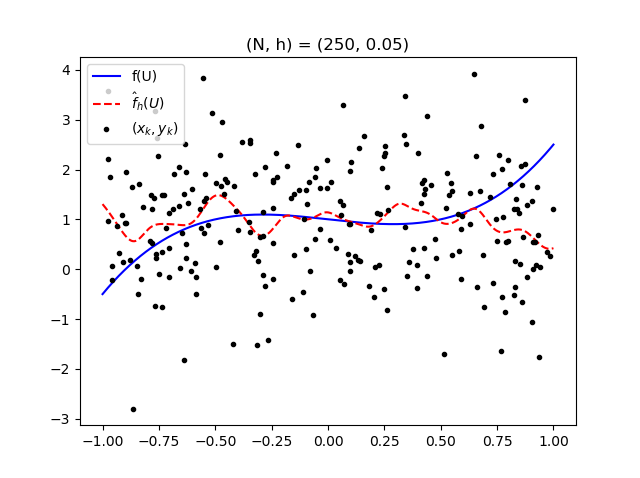
\includegraphics[height=2.4in]{Figure_5.png}
    \end{subfigure}%
    \begin{subfigure}[h]{0.5\textwidth}
        \centering
        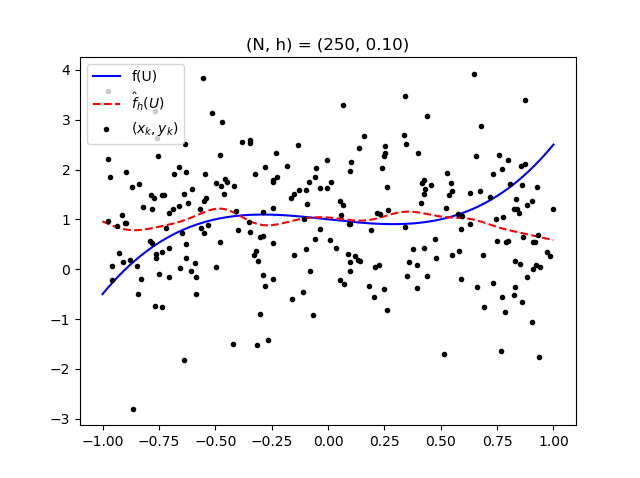
\includegraphics[height=2.4in]{Figure_6.png}
    \end{subfigure}
    \begin{subfigure}[h]{0.5\textwidth}
        \centering
        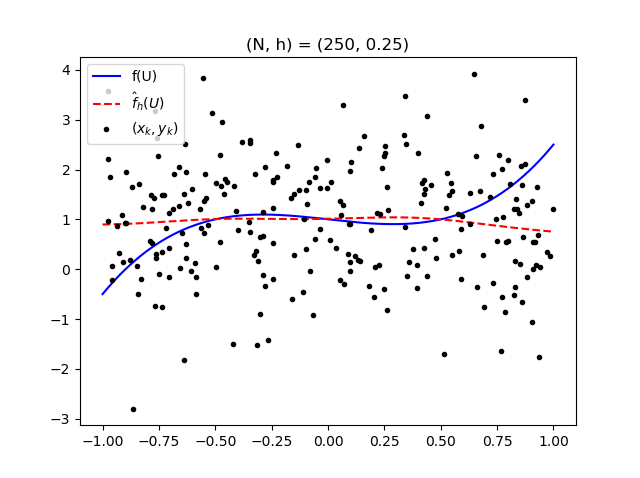
\includegraphics[height=2.4in]{Figure_7.png}
    \end{subfigure}%
    \begin{subfigure}[h]{0.5\textwidth}
        \centering
        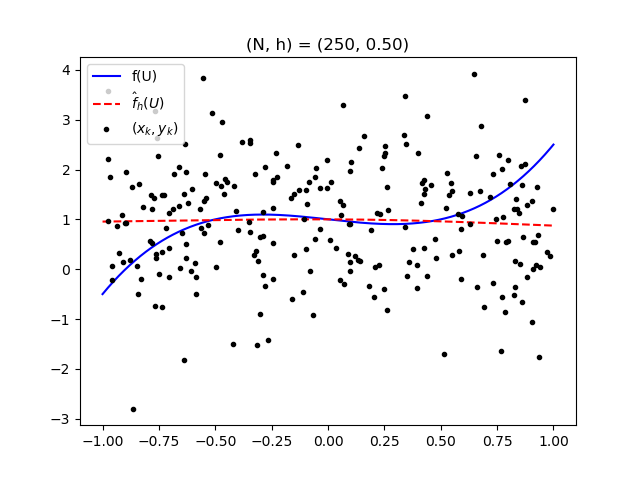
\includegraphics[height=2.4in]{Figure_8.png}
    \end{subfigure}
    \caption{Kernel regression estimators for $N$ = 250}
\end{figure}

As the kernel bandwidth increases, the variability of the calculated kernel regression estimator decreases. For each case, several error metrics were used to judge the accuracy of the kernel regression estimator. Values of $e_{1}$, $e_{2}$, and $e_{3}$ as are shown below in Table 1, alongside the error returned by 10-fold cross-validation. As the kernel bandwidth increases, $e_{1}$, $e_{2}$, and $e_{3}$ values tend to increase and the cross-validation error tends to decrease.

\begin{table}[h!]
\centering
 \begin{tabular}{||c c c c c c||} 
 \hline
 $N$ & $h$ & $e_1$ & $e_2$ & $e_3$ & $\varepsilon_{cv}$ \\ [0.5ex] 
 \hline\hline
100 & 0.05 & 1.0397 & 0.0148 & 1.0572 & 1.4899 \\
100 & 0.10 & 1.2083 & 0.0170 & 1.0693 & 1.4131 \\
100 & 0.25 & 1.3111 & 0.0572 & 1.1092 & 1.4257 \\
100 & 0.50 & 1.3304 & 0.1256 & 1.1724 & 1.3898 \\
250 & 0.05 & 1.1658 & 0.0148 & 1.0572 & 1.3342 \\
250 & 0.10 & 1.2150 & 0.0170 & 1.0693 & 1.2810 \\
250 & 0.25 & 1.2431 & 0.0572 & 1.1092 & 1.2893 \\
250 & 0.50 & 1.2519 & 0.1256 & 1.1724 & 1.2858 \\ [1ex] 
 \hline
 \end{tabular}
 \caption{Estimates of error for the kernel regression estimator}
\label{table:1}
\end{table}

(2) \(E((Y - f_{h}(X))^{2} \geq 1\), because the given standard deviation of Y is 1. If the deviation of Y was larger, the variability of the data would increase and the corresponding kernel regression estimator would also increase, resulting in a larger expected error. A similar trend can be inferred about decreasing the standard deviation of Y and having a smaller error. Of the three error metrics evaluated in Table 1, $e_{3}$ estimates this quantity the best because it calculates the error between the testing data and the kernel regression estimator. The testing data is more representative of the entire data set and the training data is only a selected subset of the generated random variable Y.